\epigraph{\textit{""}}

\paragraph{Abstract} Characterization of perovskite solar cells is a non-trivial subject, the techniques researchers successfully employed for \gls{osc} and \gls{dssc} needs to be re-validated for this new kind of solar cells. The presence of ionic migration in the absorber can be a game-changer for which special care has to be taken.

\section{Conventions and General Remarks}

	All the characterization on complete devices was performed keeping them in an air-tight holder filled with nitrogen. The electrical connection from the cell electrode to the external end of the holder was obtained using gold tips connected via a printed circuit board to a coaxial cable.

	\subsection{Sign Convention and Parameters Definitions}

		\paragraph{Fermi level} The electrons electrochemical potential, also known as Fermi level, is defined as the energy required for adding an electron in a specified position. Its value depends on the electrostatic potential $V$ in that position and on the internal chemical potential $\mu$ which in our case depends mainly on the concentration of electrons (not related to their electric charge, similarly to the density of a gas). As the Fermi level is going to be used mainly for comparisons, its zero is not going to be defined thesis-wide, instead it will be defined to a convenient reference just where needed.

		\paragraph{Cathode and anode} Considering a solar cell device at steady state under illumination and in open circuit conditions, its cathode is defined as the contact where the electrons electrochemical potential $\bar\mu$  is the highest. By consequence the other contact is the anode. The naming of the two contacts holds to the one defined in illuminated, open circuit conditions even in conditions where the contacts' electrochemical potential is in the reversed order.

		\paragraph{Voltage} The voltage $\Delta V$ is always used as a relative value, defined subtracting the electrons electrochemical potential of the cathode from the anode's one. So in the aforementioned solar cell example, the voltage is positive. The unit is the Volt.

		\paragraph{Electrical power} The electrical power $P$ is defined as positive when the device absorbs electrical energy (incoming, passive element) and negative when it generates energy (outgoing, active element). It can be expressed in extensive form with power (Watt) unit or in intensive form "electrical power density" with power over active area unit (Watt over square centimetre).

		\paragraph{Current} The current $J=P/V$ is measured through an external circuit and the sign is a consequence of the voltage and electrical power definition: A current ("conventional current", flow of positively charged particles) being released from the device's anode and being received from the device's cathode is defined as negative. This can be thought as: Inside the device, somehow, a positive charge was moved from the high Fermi level contact to the low Fermi level contact, increasing its electrochemical energy, the opposite to what would happen in a resistor, whose current is always positive. In a solar cell device, the current and the electrical power can be either positive or negative depending on the illumination and voltage conditions. It can be expressed in extensive form with current (Amperes) unit or in intensive form "current density" with current (Amperes) per active area (square centimetre) unit.

		\begin{SCfigure}
			\centering
			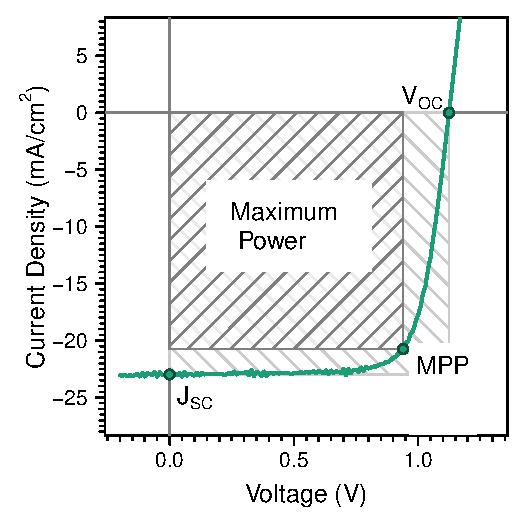
\includegraphics[width=0.5\textwidth]{iv_params/IV-revIVs.pdf}
			\mycaption[Parameters extraction from current-voltage sweeps.]{A typical current-voltage sweep is represented. MPP stands for maximum power point, \gls{jsc} stands for \glsdesc{jsc}, \gls{voc} stands for \glsdesc{voc}. The ration between the small and the large rectangles areas is the \glsdesc{ff} (\gls{ff}).}\label{fig:iv_params}
		\end{SCfigure}

		\paragraph{\Glsdesc{voc}} \Gls{voc} parameter is defined as the voltage $\Delta V$ at which the current is zero while the solar cell device is illuminated at 1~sun conditions and in steady state (positive by its own definition).

		\paragraph{\Glsdesc{jsc}} \Gls{jsc} parameter is defined as the unsigned value of the current density flowing in an external circuit short circuiting (zero resistance) the solar cell device's contacts while illuminated at 1~sun and in steady state. It is usually reported in current (milli Amperes) over active area (square centimetre) unit.

		\paragraph{Maximum power density} The maximum power density is defined as the unsigned minimum of electrical power density which can be obtained by $P(V) = J(V) \cdot V$. It is usually reported using power (Watt) over active area (square centimetre) unit.

		\paragraph{\Glsdesc{pce}} \Gls{pce} parameter is defined as the maximum power density over the illuminating power density, which at 1~sun AM 1.5G is defined to \SI{100}{\mW\per\square\cm}. It is usually reported as a percentage.

		\paragraph{\Glsdesc{ff}} \Gls{ff} parameter is defined as the ratio between \gls{pce} and the product of \gls{voc} and \gls{jsc}. This parameter does not have a physical meaning, but it represents how much the series and shunt resistances affect the device efficiency.

		\paragraph{Forward and reverse bias} Forward bias is a device condition where the voltage is positive, reverse bias is the case where the voltage is negative.

		\paragraph{Forward and reverse scan} In current-voltage sweeps, a scan where the voltage is increasing over time is a forward scan, while a voltage variation in the opposite direction constitutes a reverse scan.

		\paragraph{Ideality factor} An ideality factor $m$ different from 1 describes deviations from the ideal photo-diode. The adapted $J(V,\phi)$ equation becomes\cite{Calado2018b}:
		\begin{equation} \label{eq:photodiode}
			J = J_{SC}(\phi) - J_0\left(\exp\left(\frac{qV}{mk_BT}\right)-1\right)
		\end{equation}
		where $J_0$ is the diode saturation current (the current flowing in dark when applying a reverse bias), $q$ is the elementary charge, $k_B$ is the Boltzmann constant, and $T$ is the temperature.  Clearly the reported equation just offers a simplified model. For example, it can be improved adding the contribution from the series resistance $R_s$ and would become

		$$J = J_{ph}(\phi) - J_0\left(\exp\left(\frac{q(V+JR_s)}{mk_BT}\right)-1\right)$$

		where now $J_{ph}$ is the total photo-generated current. The function is now an implicit one, requiring numerical solving even for obtaining $J_{SC}$.

		\paragraph{Top and bottom of devices} The point of view of the manufacturer is used for defining the physical top and bottom of a device: the bottom is the glass substrate and the top is the last deposited layer. This is opposite with the usage of a solar cell in the real world and with most of the solar simulators (but not all of them, for example Paios from Fluxim has an illumination from below, more convenient for contacting the electrodes without a samples holderCITE FLUXIM).

	\subsection{Usage of Shadowing Mask}

		\begin{SCfigure}
			\centering
			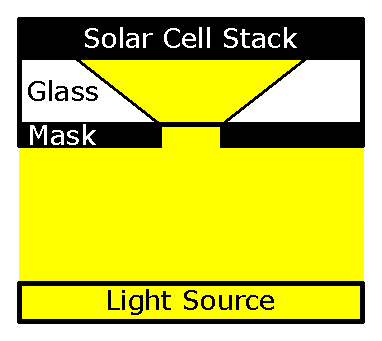
\includegraphics[width=0.5\textwidth]{shadowing_mask/shadowing_mask.pdf}
			\mycaption[Illuminated area after a shadowing mask.]{This schema is just for explaining the concept described in the text, its dimensions are not realistic.}\label{fig:shadowing_mask}
		\end{SCfigure}

		In literature is generally suggested to use a shadowing mask when measuring the solar cell devices in order to better define the illuminated area (as in the brokenCITE BRINSER form from Nature\cite{NatureResearch2017}). %, the file is a dynamic XFA form and cannot be opened by most PDF readers (and they rightly do not, as it was deprecated in ISO 32000-2:2017), Adobe products or Master PDF Editor is required for reading).
		In our case the active area is just \SI{0.09}{\square\cm} so the mask aperture should be extremely small and its exact positioning troublesome. Additionally, the fact that the illumination reaches the mask from a wide angle (the illuminating source dimension, which is not just the lamp as the illumination passes through spread lenses, is not small compared to the lamp-cell distance) allows the light to spread through the substrate glass (\SI{2.2}{\mm} for \gls{fto} substrates, other groups use even thicker glass substrates) reaching a significantly larger area on the active layer at the other side of the glass, as represented in \cref{fig:shadowing_mask}. In our solar simulator a linear widening of 8~\% over \SI{2}{\mm} was estimated, this makes an illuminated area 16~\% larger than the mask aperture. Even if the total incident power is still determined from the mask aperture, the illumination intensity is not 1~sun any more, compromising the validity of a measurement done with a shadowing mask.


	\subsection{Stability During the Measurement and Small/Large Perturbations}

		Most of the reported hybrid lead halide perovskite materials can show rather impressive changes in their structure on long time scales, for example due to ionic migration CITE, degradation CITE and self-healing CITE 10.1002/adma.201706273.
		This have to be taken into account for all the measurements techniques output which either takes too long time to be measured or employs large perturbations.

		\paragraph{Long lasting measurement} An example of the first case is the impedance spectroscopy where during the long lasting measurement various phenomena can occur, like: a slow current evolution due to perovskite well known hysteretic behaviour prior to stabilization; a degradation process changing the current; the heating of the device changing its properties. This slow current evolution can easily be misinterpreted for capacitive current CITE JACOBS and introduce artefacts like loops in the Nyquist plots CITE IMPEDANCE PAPER.

		\paragraph{Large perturbations} Large perturbations regime means that the independent variable being perturbed is changed by an amount large enough to cause the quantities under study to not follow the approximation given by the first term of the series expansion. Let's take some example.

		\paragraph{Large perturbations -- \gls{tpv}} For example, if too intense, the light pulse in \acr{tpv} could change the voltage by a less-than-linear amount. In this case, the light pulse is not only probing the recombination, but it is adding some, so a large perturbation has to be avoided.

		\paragraph{Large perturbations -- impedance} Another example: a too wide sinusoidal voltage oscillation amplitude in impedance measurements can cause a non-sinusoidal current output. This is not a problem for the measurement itself, as the lock-in amplifiers are perfectly able to extract the amplitude and the phase of the signal first harmonic, ignoring the higher harmonics caused by the too large perturbation. But artefacts could arise and cause misinterpretations, as explained in \cpageref{impedance-large_perturbations}.

		\paragraph{Large perturbations -- \gls{trpl}} Last example: in the \glsdesc{trpl} a laser pulse illuminates the otherwise unilluminated absorber layer. This pulse induces a the migration of the ionic defects to a new profile depending on the pulse intensity CITE LEVINE 2018 ARXIV, by a small extent due to its short duration. The fact that the relaxation time of the ionic migration is usually much larger than the laser repetition rate (\si{\ms} to seconds for the ionsCITE JACOBS and \si{\ms} to \si{\us} for typical \gls{trpl} lasersCITE EDINBURGH) implies that the ionic profile variation slowly "builds up" pulse after pulse. As the ionic profile affects the free charges concentration, and this in turn rules the radiative recombination, the measurements of \gls{trpl} have to be done with extreme care. An example of hysteretic behaviour observed with \gls{trpl} can be found in CITE AUTHORYEAR 10.1021/acsenergylett.6b00355 .


\section{Current-Voltage Sweeps}

	After calibrating the light intensity in the solar simulator (see \cpageref{solarsimulator}), the devices were exposed to the illumination at open circuit for some seconds in order to have a stabilized open circuit voltage. Then usually the curves were measured with the auto-measure function of the PyPV software (see \cpageref{automeasure}) which measures the reverse scan and then the forward scan.

	\paragraph{Parameters Extraction from Sweeps}
	For the devices studied in this thesis, the reported values of \gls{voc}, \gls{jsc}, \gls{pce} and \gls{ff} are extracted from a forward or reverse current-voltage sweep. This is in accordion to the tradition of solar cells reporting but for hysteretic devices, like perovskite solar cells, a static measurement should be preferred. %Checking the aforementioned definitions, one can easily notice how this is not the correct way as these parameters need to be measured in steady-state conditions. This is comes from the tradition of solar cell reporting, which was established in pre-hysteresis times and is no longer a valid approximation. Apologizing for the lack of coherence I hope I'll be able to implement the static measurements of \gls{voc} and \gls{jsc} in the PyPV measurement routines (described in \cpageref{automeasure}).

	\paragraph{Parameters Extraction from Sweeps -- \gls{pce}} Regarding the \gls{pce}, and by consequence the \gls{ff}, a proper measurement is made difficult due to the cell evolution over time (hysteresis). The voltage associated to the maximum power point is drifting and its localization affects its evolution. A proper \gls{mppt} system needs to be bought or developed, see \cpageref{software_mppt} for thoughts about possible implementations.

	\paragraph{Auto-scale}\label{autoscale} In literature one can easily find current-voltage curves with discontinuities or "kinks"\cite{Li2016,Snaith2014,Zhang2015} CITE  10.1039/C4MH00238E  like the one reported in \cref{fig:autoscale}. Some even lucubrate about the origin of these in perovskite solar cells. Indeed this is likely just caused by the auto-scale feature of the Keithley equipment, disabling this, the discontinuities disappears.

	\begin{SCfigure}%[!hbtp]%
		\centering
		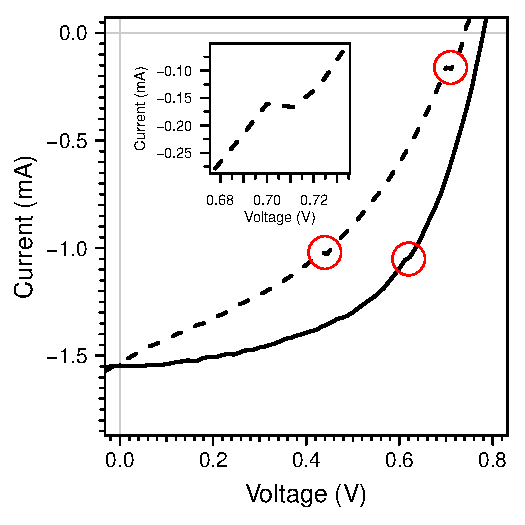
\includegraphics[width=0.5\textwidth]{autoscale/ig1-3-1-int4.pdf}
		\mycaption[Kinks in JV sweep due to autoscale.]{A current-voltage sweep of an hysteretic perovskite solar cell with Keithley autoscale active. Both the forward (dashed) and the reverse (solid line) present small discontinuities around \SI{1}{\mA} and \SI{0.1}{\mA}.}\label{fig:autoscale}
	\end{SCfigure}

	\paragraph{Scan speed} The used sweep speed is \SI{500}{\mV\per\s}, which was arbitrarily chosen for avoiding bumps leading to currents higher than \gls{jsc}, like the one in \cref{fig:iv_ugly}. %having an aesthetically good looking current-voltage curve
	Our arbitrary choice allowed us to make fair comparisons between devices, but the absolute values should be considered as approximations.
	\begin{SCfigure}%[!hbtp]%
		\centering
		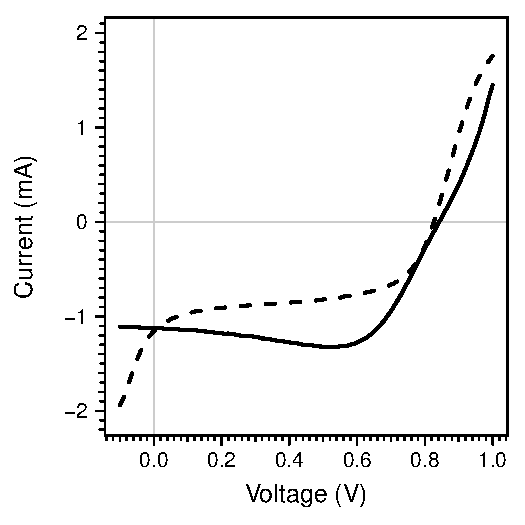
\includegraphics[width=0.5\textwidth]{iv_ugly/ig47-b32-int2-4.pdf}
		\mycaption[Hysteretic current-voltage scan.]{At the employed scan speed, the hysteresis phenomena causes the reverse (solid line) scan to reach currents higher than the \gls{jsc}.}\label{fig:iv_ugly}
	\end{SCfigure}
	We wanted to underline that due to hysteresis phenomena, no scan speed, direction, or precondition is the correct one.  % and they all heavily affect the resulting \gls{pce}.
	Rather, a static measurement or a \acr{mppt} should be used for obtaining a accurate and realistic result.
	This comment regards also the so-called "hysteresis-free" perovskite solar cells, which can also have hysteretic phenomena\cite{Jacobs2018}.

	\paragraph{Noise} The noise often observed in current-voltage sweeps at high scan speeds in this thesis is mainly caused by oscillations in the solar simulator illumination intensity, as an example see \cref{fig:iv_params}. For reducing the noise impact on the \gls{jsc} and \gls{voc} parameters extraction, these values were extracted via a parabolic fitting. %Indeed, using a white \gls{led} as illumination source, this noise is not present but the spectral mismatch affects the meaningfulness of the measurement.

	\paragraph{Stabilized or dynamic current-voltage sweeps} One very appealing alternative to current-voltage sweeps are the so-called "stabilized current-voltage sweeps", where at each voltage point a fixed stabilization time is waited and the stabilised current is reported. CITE 10.1039/c4ee02465f 10.3390/photonics2041101
	An improvement of this technique is named "dynamic current-voltage sweeps", here the stabilization step is of variable duration, until the current-time derivative falls below a threshold (e.g. \SI{0.2}{\%\per\minute}).CITE 10.1039/c7ta05609e 10.1002/pip.2839
	In this thesis, these techniques have not been used.

	\paragraph{Shunt and series resistances} \label{resistances} In our group the shunt and series resistances are evaluated by the current versus voltage derivative of a dark current-voltage sweep respectively at zero and at high-enough voltage. This methodology is inherited from organic solar cells and, as is easy to foresee, is unreliable on hysteretic devices: in the case of perovskite solar cells a measurement of the stabilised current at a few points have better chances to produce a useful result. The measurement of the current at a voltage close to zero is enough for estimating the shunt resistance while two points at high voltages are needed for estimating the series resistance.

\section{V\textsubscript{OC} and J\textsubscript{SC} Dependence on Light Intensity}
	The solar simulator illumination intensity $\phi$ is reduced via neutral density filters with transmittance of 0.05, 0.12, 0.25, 0.51, 0.81 and 1 (no filter). The values of $V_{OC}(\phi)$ and $J_{SC}(\phi)$ can be obtained from static measurements or from current-voltage sweeps. The static measurement of $V_{OC}(\phi)$ at high light intensities is troublesome as it can easily damage the device. In this thesis, the used method is specified case by case. %this measurement is reported both from static measurement of \gls{voc} and from \gls{voc} obtained from current-voltage sweeps; the used method is specified case by case. %The devices are kept at this reduced illumination $\phi$ and at open circuit or short circuit conditions until steady state for measuring respectively 

	\subsection{\Gls{jsc} versus $\phi$}
		The \gls{jsc} dependency on the light intensity $\phi$ is close to linear and can be fitted with a power law:
		\begin{equation} \label{eq:jsc-phi}
			J_{SC} \propto \phi^\alpha
		\end{equation}
		giving $\alpha$ values usually from 0.95 to 1.

		\paragraph{Interpretation} %The \gls{jsc} dependency on the light intensity $\phi$ is close to linear and can be fitted with a power law $J_{SC} \propto \phi^\alpha$ as described in \cpageref{methods_jsc_intensity}.
		An $\alpha$ value lower than 1 indicates the presence of non-geminate recombination (for geminate recombination see \cpageref{intro_geminate}) at short circuit\cite{Credgington2011}, indicating that not all the photo-generated charges get extracted, neither at short circuit conditions.

	\subsection{\Gls{voc} versus $\phi$ and the Ideality Factor $m$}

		Setting $J=0$, which corresponds to open circuit conditions, in \cref{eq:photodiode} (without considering the series resistance correction) we can obtain a relation between \gls{jsc} and \gls{voc}:
		%\begin{equation} \label{eq:photodiode-zerocurrent}
		$$J_{SC}(\phi) = J_0\left(\exp\left(\frac{qV_{OC}(\phi)}{mk_BT}\right)-1\right)$$
		%\end{equation}
		This equation can already be used for obtaining the $m$ and $J_0$ values fitting the \gls{jsc} and \gls{voc} measured at different light intensities $\phi$ (also varying the temperature could be used for fitting the values, but it was not done during this thesis).

		Solving for \gls{voc} we obtain:
		%\begin{equation} \label{eq:photodiode-zerocurrent-voc}
		$$V_{OC}(\phi) = \frac{mk_BT}{q}\cdot\ln\left(\frac{J_{SC}}{J_0} + 1\right)$$
		%\end{equation}

		Considering that the saturation current $J_0$ (current in dark under reverse bias) is much smaller than $J_{SC}$ for the light intensities we usually employ (down to \SI{0.05}{suns}), we can approximate to:
		%\begin{equation} \label{eq:photodiode-zerocurrent-voc_approx}
		$$V_{OC}(\phi) \approx u_1 + \frac{mk_BT}{q}\cdot\ln(J_{SC})$$
		%\end{equation}

		where $u_1$ is a useless constant. Then if the $\alpha$ value is close enough to~1, we can use \cref{eq:jsc-phi} and further approximate for plotting against light intensity $\phi$:

		$$V_{OC}(\phi) \approx u_2 + \frac{mk_BT}{q}\cdot\ln(\phi)$$

		This is the equation we commonly employ for fitting and obtaining ideality factorsCITE NELSON CITE Kirchartz2012. %In literature one can found reports of ideality factor determined via \gls{voc} versus \gls{jsc} dependency. The results of the latter method may differ from the aforementioned one due to series resistance and the non-linear dependency of the \gls{jsc} from the light intensity ($\alpha < 1$). 
		The so-obtained ideality factor $m$ is usually from 1 to 2. A voltage dependent ideality factor can also be measured from a current-voltage sweeps in dark but has not been evaluated in this thesis, as it would be affected by hysteresis. A critical analysis of these methods and the proposal of a new "Transient Suns-\gls{voc}" method (employing a pre-biassing for flattening the ionic profile) can be found in \authoryear{Calado2018b}. % Anyway in perovskite solar cells exhibiting hysteresis, a current-voltage sweep would not give fair ideality factors and the current-voltage points should be acquired reaching steady state conditions for each point. Both these methods for deriving the ideality factor have been implemented in the DrIFtFUSION simulation as described in \cpageref{dd_ideality}.

		\paragraph{Interpretation} %\The \gls{voc} dependency on the light intensity $\phi$ can be fitted with a natural logarithmic dependence obtaining the ideality factor $m$. 
		\authoryear{Pockett2015} measured ideality factors of planar perovskite solar cells via stabilized \gls{voc} obtaining, for some cases, values as high as 5. Also in organicCITEKirchartz2011 CITEKirchartz2012 and silicon solar cellsCITE Breitenstein2006 ideality factors greater than 2 has been observed and explained. According to \authoryear{Calado2018b}, the ideality factor, once obtained in the correct way, is 1 when studying most of the recombination types and 2 for mid-gap trap mediated recombination in regions where the electrons and holes concentrations are similar, $n \approx p$.

\section{Charge Extraction (CE)}

	The device is kept under 1~sun equivalent illumination by a white \gls{led} at open circuit conditions until stabilization is reached. 1~sun equivalent illumination is defined as the illumination at which the a silicon photodiode gives the same \gls{jsc} as under calibrated 1~sun from the solar simulator. The \gls{led}-solar spectral mismatch affects slightly the measurement, but in no case a \gls{pce} is reported from any \gls{led}-illuminated experiment. After stabilization the illumination is switched off and, at the exactly same moment, the device is short circuited through a small and known resistance of \SI{50}{\ohm} \cite{Duffy2000}.

	This is repeated decreasing the light intensity from 1~sun down to dark (in dark no signal should be observed, indeed some residual charge can usually be seen, the reason of this could be ionic profile updating or an insufficient darkness) and a single decay is measured for each illumination point, over approximatively 30 illumination points.

	The equipment includes two transistors (in a home made circuit by Dr. Javier Pérez Hernández) connected to a pulse generator providing a square pulse long at least as the measurement window. From my experience, I recommend to use a short dark period in order to save time for the following stabilization step.

	The measurement is carried out with an oscilloscope in parallel to the known small resistance. In the first microseconds, most of the free charge flows through the resistor generating a voltage drop across it which is measured by the oscilloscope. This potential drop can be converted to current using the Ohm's law, which, integrated over time, gives the amount of extracted charge.

	\paragraph{Noise reduction}\label{r_ce_noise}
	Most of the observed short-times noise (\SI{< 5E-7}{\s}) is, supposedly, related to the opening and closing of the transistors included in the in-house built circuit.

	Annoyingly, the noise profile is characteristic of the cell and of the circuitry, so a simple average over many decays does not help in cancelling it.

	This affects the resulting measurement to a noticeable extent, which starts to be a problem if the charge versus light bias (\gls{voc} generated at a given illumination intensity) profile has to be studied in detail, as in \cref{ch:tae}.

	In order to reduce this effect various approaches have been tested; finally the single decays were fitted with a bi-exponential formula (sum of two exponential) and the integral of this fit was used.
	
	For the implementation, see \cpageref{r_ce}.

\section{Interpretation of Charge Extraction}\label{interpretation_ce}
\paragraph{\Acr{ce} time constant}
The free charges extraction time is related to the RC time of the \SI{50}{\ohm} resistor and the capacitance of the solar cell device. We can see in \cref{fig:chargeExtraction_RCtime} a weak covariance (Pearson correlation coefficient of 0.3) between the RC time obtained considering the dark capacitance from \acr{dc} (geometric capacitance) and the extraction time (as obtained by an exponential fitting to a single \acr{ce} current decay) at low light intensity (enough for having a signal but far from 1~sun light intensity). At higher light intensities, the correlation is weaker as the capacitance is less defined as the cell is in a transition between illuminated (high capacitance) and dark (low capacitance) status. Anyway, the extraction time does not change much between low light intensity and 1~sun with an increase from \SIrange{1.1}{2.4}{times} (first and third quartile).

\begin{SCfigure}%[!hbtp]%
	\centering
	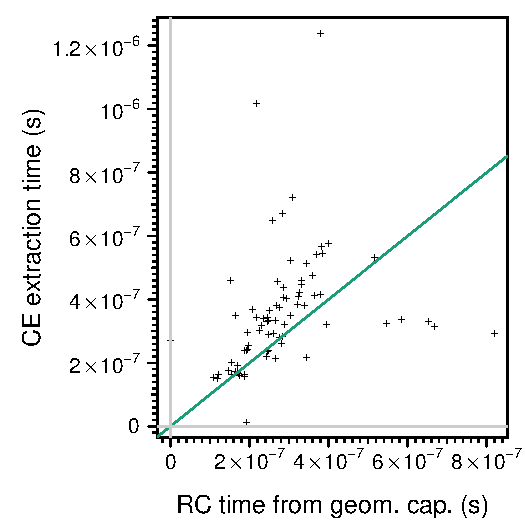
\includegraphics[width=0.45\textwidth]{chargeExtraction_RCtime/CEaBitOfSunExpTime_vs_RCdarkTime.pdf}
	\mycaption[Charge extraction time is related to a RC time.]{Covariance of \acr{ce} extraction time at low light intensity versus the expected time from geometric capacitance (as obtained from dark \acr{dc}). Each point is a different device, many different structures studied during my PhD are represented. The grey line indicates the 1 to 1 relationship.}\label{fig:chargeExtraction_RCtime}
\end{SCfigure}

\paragraph{Comparison between \acr{ce} time constant and \acr{tpv} time constant}
During this time, and depending on its location in the device stack, some free charge can recombine. One could argue that a \acr{ce} measurement is valid only if the extraction is faster than the recombination time as measured via \acr{tpv}CITE RYAN2017 or that the extracted charge should be corrected considering the recombination CITE Credgington2011. Considering the charges accumulated in the depletion layers in the selective contacts, these will flow to the electrodes without crossing the perovskite/selective contacts interfaces, where has been reported that most of the recombination occurs CITE 10.1021/jz501163r CITE Stolterfoht2018a CITE Stolterfoht2018. So this part of the extracted charge, distinguishable as the linear part of the charge versus voltage plot, as represented in \cref{fig:} should not be corrected. Instead, regarding the charge accumulating in the perovskite layer, which we assume can be assigned to a chemical capacitance and can be recognized as the exponential part in \cref{fig:}, it may be that a correction CITE 10.1063/1.3006316 EPAPS Document No. E-APPLAB-93-043843 is needed, but this has not be done in this thesis.

\paragraph{Interpretation of the single measurement}
From some preliminary and unpublished simulations of \acr{ce} show that a short living exponential decay can be accounted for free charges and a long living and weak exponential decay is caused by a displacement current due to ionic profile updating to the new voltage. The slow decay is not usually measured and seldom reported\cite{ORegan2015b}.

\paragraph{Interpretation of the charge versus light bias trend}



\section{Transient PhotoVoltage (TPV)}
	\epigraph{\textit{"Imma firin mah lazor\\pewpew pewpewpew"}}

	The device is kept under 1~sun illumination by a white \gls{led} ring at open circuit until stabilization is reached. 1~sun equivalent illumination is defined as the illumination at which the a silicon photodiode gives the same \gls{jsc} as under calibrated 1~sun from the solar simulator. Then an additional illumination pulse is provided by a nitrogen laser. The pulse duration is around \SI{1.5}{\ns}. The equipment can output up to 20~pulses per second, but due to the oscilloscope settings and oscilloscope internal memory speed we're limited to 1~pulse per second (maybe decreasing the number of acquired points would allow us to acquire higher repetition rates). The pulse was triggered with a square wave pulse generator. The wavelength is selected with the absorption and emission of a dissolved molecular dye, usually a wavelength of \SI{650}{\nm} is selected using a RhodamineB solution\cite{RadiantDyesLaser}, this wavelength allow us to illuminate in deep the perovskite layer (in contrast to a blue light where the illumination would be absorbed within the first hundreds of nanometres of the material).

	During all the process, the device is connected to a \SI{1}{\Mohm} oscilloscope, registering the open circuit voltage profile (the high resistance of the oscilloscope is a good approximation of open circuit). An auxiliary output from the square wave pulse generator used for the pulse is used for the trigger of the oscilloscope.

	The intensity of the laser pulse is decreased using a variable neutral density filter (a partially reflecting wheel with different positions for different transmittivities) so that the voltage perturbation caused by the light pulse does not exceed \SI{10}{\mV} with 1~sun background illumination intensity. We consider this as a "small-enough" perturbation.

	This process is repeated decreasing the light intensity from 1~sun down to dark. Clearly, the pulse intensity which could be considered a "small-enough" perturbation at high background illumination is not so at lower ones and cannot be small at dark conditions. We \emph{do not} regulate the pulse intensity depending from the background illumination for being able to use this data also for \acr{dc} studies. The \acr{dc} does not intrinsically need the usage of a constant pulse intensity but it needs the measurement of a \acr{tpc} for each pulse intensity. The switch from \acr{tpv} to \acr{tpc} setups and back would be complex and time demanding with the current setup. Anyway quite all the information from the \acr{tpv} is obtained from the high background illumination intensity measurements.

	For each illumination intensity, the reported decay is the result of averaging around 30~transients. This manages to reduce the noise.

	For the interpretation, see \cpageref{interpretation_tpv}; for the implementation, see \cpageref{r_tpv}.


	\paragraph{Noise treatment}\label{tpv_robust}

	Most of the observed noise (\SI{< 2E-7}{\s}) is due to the radiofrequency emitted by the spark in the nitrogen laser which gets absorbed by all the non-coaxial cables (coaxial ones don't) and from the circuitry of the samples holder acting as a receiving antenna. On the contrary to what happens for \acr{ce}, the short times noise seems to not follow a constant pattern, so averaging the measurement over a few repetitions (usually 30) manages to reduce the noise.

	This noise can affect the exponential or bi-exponential fitting, for this reason a robust fitting routine has been used, which gives a lower weight to outlier points. An example can be seen in \cref{fig:tpv_robust}.

	\begin{figure}
		\centering
		\includegraphics[width=0.9\textwidth]{{tpv_robust/TPV_ig52-68-3_0.883897_V-monoexp}.pdf}
		\mycaption[Robust and normal fitting comparison.]{In grey the fitted points, in yellow the points not considered for the fitting, the solid black line is the \gls{loess}. The normal non-linear least squares fitting (in green) is affected by noise, outliers and characteristics not of interest by the model. The non-linear robust fitting (in brown) manages to reduce the weight of these points.}\label{fig:tpv_robust}
	\end{figure}


	\paragraph{Voltage Increase Value}\label{tpv_deltaV}

	The value of the voltage increase due to the additional illumination is needed for \acr{dc} measurement.

	In the group this $\Delta V$ value was traditionally obtained subtracting the steady state \gls{voc} from the maximum voltage point in the measured transient. This is obviously heavily affected by the aforementioned noise when a short time window is used.

	The following alternatives were tested:
	\begin{itemize}
		\item The linear factor in an exponential fit was used, but it can fail if the decay does not have a simple exponential shape (often a bi-exponential, sum of two exponentials, is observed);
		\item The sum of the two linear factors in a bi-exponential fit, which could work but one have to carefully set boundary values to the fitting parameters for avoiding a fast exponential matching just some noise;
		\item The maximum value of a \gls{loess} local regression was used, but this underestimates the value, especially when the peak top are just few points (when the measurement time window is large);
		\item The average of the values registered starting from the maximum voltage point and during a specified time lapse.
	\end{itemize}

	This last option is the one currently in place. The average was performed over \SI{50}{ns} after the peak and this allowed us to get a reliable $\Delta V$ value.

\section{Interpretation of Transient PhotoVoltage}\label{interpretation_tpv}

\paragraph{Factors Affecting the \acr{tpv}}
The decays we can observe are limited at long times by the discharge of the extra charge through the oscilloscope resistance and through the device shunt resistance, whatever is the smallest. This happens with an RC time of the circuit composed by the capacitance of the device and the \SI{1}{\Mohm} resistance of the oscilloscope or the internal device resistance. The oscilloscope resistance could be varied using an attenuating probe (usually 10X or 100X). This limit to long times is often observed at low light intensities as a plateau in the \acr{tpv} graph. XXXXXXXXXXXXXXXXXXXXXXXXXXXXXXXXXXXXXXXXXXXXXXXXXXXXXXXXXXXXXXXXXXXXXXXXXXXXXXXXX

\begin{SCfigure}
	\centering
	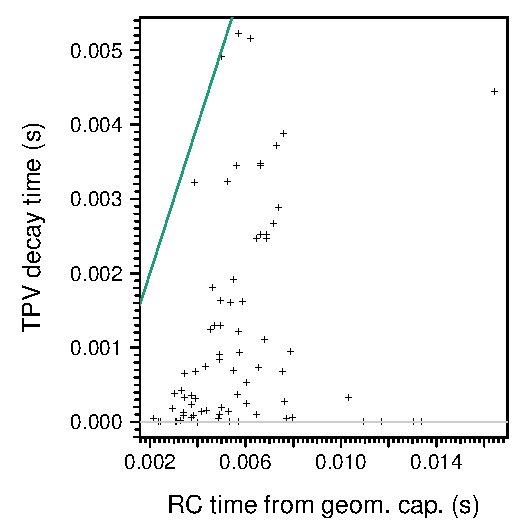
\includegraphics[width=0.45\textwidth]{tpv_RCtime/TPVdarkTime_vs_RCdarkTime.pdf}
	\mycaption[\gls{tpv} time has an upper bond due to discharge through oscilloscope.]{The green line indicates the 1 to 1 relation between the dark \acr{tpv} time (from a robust exponential fit) and the RC time derived from the geometric capacitance from \acr{dc} and the \SI{1}{\Mohm} of the oscilloscope. Each point is a different device.}\label{fig:tpv_RCtime}
\end{SCfigure}

\section{Interpretation of Transient PhotoVoltage Referenced to Charge Extraction}\label{interpretation_tpvce}

recombination order $\Phi = \lambda + 1$ CITE 10.1103/PhysRevB.78.113201 Credgington2011



\section{Transient PhotoCurrent (TPC)}

	The device is kept under 1~sun illumination by a white \gls{led} ring at short circuited through a \SI{50}{\ohm} resistor until stabilization is reached. 1~sun equivalent illumination is defined as the illumination at which the a silicon photodiode gives the same \gls{jsc} as under calibrated 1~sun from the solar simulator. Then an additional illumination pulse is provided by a nitrogen laser.

	The signal is acquired by an oscilloscope in parallel to the \SI{50}{\ohm} resistor. This allows us to measure a potential drop across the resistor and the related current via Ohm's law. Subtracting the constant current due to the background illumination and integrating the transient over time gives the charge generated by the laser pulse.

	This process is repeated at 1~sun and at dark background illumination conditions.

	For each illumination intensity, the reported decay is the result of averaging around 30~transients. This manages to reduce the noise.

	For the interpretation, see \cpageref{interpretation_tpc}; for the implementation, see \cpageref{r_tpc}.

\section{Differential Capacitance (DC)}

	This is a meta-measurement as it just combines the data from \acr{tpv} and \acr{tpc} without requiring any additional experiment\cite{Shuttle2008}, sometimes also referred to as "differential capacitance".

	As explained in \cpageref{interpretation_dc}, the electrical capacitance of a solar cell is not a constant (as in most of the commercial capacitors), indeed it depends on the applied voltage bias or light bias.

	The charge obtained with the \acr{tpc} (in case the dark and illuminated results were different, the third quartile of all \acr{tpc} measurements was used) is divided by an array of values obtained from \acr{tpv}, one for each illumination intensity. The needed value is the \gls{voc} increase due to the laser pulse, prior to the decay to steady state, for each illumination intensity (obtained as described in \cpageref{tpv_deltaV}).

	This allows us to estimate the capacitance of the solar cell device at open circuit with various illumination intensities.

	For the interpretation, see \cpageref{interpretation_tpc}; for the implementation, see \cpageref{r_tpc}.

\section{Impedance Spectroscopy}

\section{Stark Spectroscopy (ElectroAbsorbance)}

\section{Interpretation of Kelvin Probe Force Microscopy}\label{interpretation_kpfm}

\section{Molecular Characterization}
\subsection{Interpretation of Band Gap Values Obtained via Tauc Plot, PhotoLuminescence and Computational Simulations}\label{interpretation_bg}

	Otra cosa, flipé mucho con la respuesta del Vidal y me puse a intentar
	ver que se supone que se saca del espectro experimental y desde cual
	pico. Como el dijo, las simulaciones son correctas.
	Pero, creo que sea mi concepto (el HOMO-LUMO está bastante lejos del
	absorption onset, como demostrado de sus simulaciones donde el
	absoprtion onset, por ejemplo de TAE-1, está a 2.9 eV y el HOMO-LUMO gap
	está a 5.06 eV) que lo de Vidal (el pico de máxima absorción no tiene
	nada a que ver con el HOMO-LUMO gap, en mi opinión para nada) estaban
	totalmente equivocados y que habría que enviar a medir el UPS de las
	moléculas para sacar el HOMO-LUMO gap.

	El concepto está explicado en el primer párrafo de esta pagina:
	https://chemical-quantum-images.blogspot.com/2013/06/why-is-homo-lumo-gap-not-good-guess-of.html

	Lo que he puesto, o sea que lo hemos medido por Tauc plot, creo colaría
	porque todo el mundo lo mide así y está bien aceptado como método. Pero
	la verdad es que es valido solo para semiconductores donde los orbitales
	están bien deslocalizados, no como nuestra molécula en solución donde el
	estado es bien localizado en la molécula.

\section{Our Solar Cells Characterization Steps}

	In this section I'll describe the routinary characterization performed in Palomares group.


